%************************************************
\chapter{Introducción}\label{ch:introduccion}
% ************************************************

La mecánica cuántica es un área de la física que describe sistemas a escalas atómicas. Dado que en la Física, como en las ciencias en general, gran importancia de una teoría radica en su poder de predecir, el entendimiento de la mecánica cuántica fue cuestionado por las personas de la época en sus inicios (1920's), pues sus fundamentos eran ideas revolucionarias contra intuitivas con la descripción de la naturaleza que ofrecía la mecánica que hasta entonces se conocía: la mecánica clásica, pues en esta última, dado un sistema y sus condiciones iniciales, preguntas como: ¿Dónde estará la partícula al tiempo $t$?, tenían una respuesta concreta que podía ser comprobada mediante experimentos. La mecánica cuántica por otro lado, plantea una respuesta en términos de una densidad de probabilidad, en donde, hasta hacer una medición, podremos saber con exactitud la posición de una partícula.
\\
La interpretación de la mecánica cuántica sigue siendo un tema que genera discusión, sin embargo, la validez y fortaleza de la teoría no son puestas en duda, pues es capaz de explicar el comportamiento de las partículas a pequeña escala, así como sus interacciones, de manera exitosa y de acuerdo a las pruebas experimentales.
\\

La evolución temporal de un sistema cuántico es de gran interés para diversas áreas de la ciencia, pues tiene diversas aplicaciones para procesos químicos y biológicos. En tales procesos es importante tener una descripción cuántica del sistema, ya que trata de interacciones a niveles atómicos o moleculares. La Ecuación de Schrödinger Dependiente del Tiempo, \acs{TDSE}, por sus siglas en inglés, es la ecuación que describe la evolución temporal de un sistema cuántico; por otro lado, el Hamiltoniano de un sistema, en el formalismo de la mecánica cuántica, es un operador que contiene la información de la energía total del sistema.
\\
La solución a la ecuación de Schrödinger depende del Hamiltoniano del sistema, y cuando el Hamiltoniano tiene una dependencia temporal, como es el caso de muchos sistemas de procesos químicos, adquiere una forma más compleja dependiendo del sistema. Para resolver la \acs{TDSE} y encontrar una descripción de la evolución del sistema, se pueden emplear diversos métodos analíticos o numéricos; sin embargo, dependiendo de la naturaleza del sistema, los cálculos y su tiempo de cómputo pueden llegar a representar un problema para obtener resultados de manera eficiente.
\\
\\
En los últimos años, las Redes Neuronales Artificiales \acp{ANN} por sus siglas en inglés, han sido modelos de Aprendizaje Automático que han cobrado popularidad debido a los avances en computación, al uso de Unidades de Procesamiento Gráfico (GPU's), al mejoramiento en algoritmos y modelos; y al incremento de datos. Actualmente, en diversos problemas, pueden ofrecer resultados que consumen menos tiempo y/o memoria de cómputo, con una precisión exitosa. De la manera más general, las \acp{ANN} pueden verse como gráficas computacionales de operaciones matemáticas, cuya forma de aprender\footnote{Históricamente las \acp{ANN} fueron inspiradas por las estructuras neuronales biológicas; un concepto como el \emph{entrenamiento} de una \acs{ANN}, puede interpretarse como el proceso análogo de \emph{aprendizaje} que tienen los organismos biológicos.} se basa en procesar ejemplos de datos referentes al problema o sistema en cuestión.
\\
\\
El objetivo de este trabajo es la implementación de una \acs{ANN} que funcione como propagador para cierto tipo de sistemas cuánticos, es decir, que mapee una función de onda en un tiempo inicial $t$: $\psi(r,t)$, a la función de onda después de un intervalo de tiempo $\Delta t$: $\psi(r,t+\Delta t)$, bajo condiciones iniciales que dependen del sistema, obteniendo así, un modelo alternativo a los métodos analíticos y numéricos para la resolución de la \acs{TDSE} para este tipo de sistemas.

\section{Organización}

En la segunda parte de la tesis (\autoref{pt:TDSE}) se abordan conceptos básicos de Dinámica Cuántica y la Ecuación de Schrödinger Dependiente del Tiempo (\acs{TDSE}) para la descripción de la evolución temporal de sistemas cuánticos. En el \autoref{ch:DVR} se desarrolla un ejemplo de método numérico para la resolución de la \acs{TDSE} aplicada al tipo de sistemas cuánticos de interés para este trabajo.\\

La tercera parte de la tesis (\autoref{pt:ANNS}) describe una breve introducción sobre Aprendizaje Automático y aprendizaje supervisado, posteriormente se describen los fundamentos y características principales de las redes neuronales artificiales (\acp{ANN}).\\

La última parte de la tesis (\autoref{pt:Modelos}), detalla la implementación de un modelo particular de \acs{ANN} como propagador aplicado a los sistemas cuánticos de interés (\autoref{sec:ProtonTransfer}); la obtención y manejo de datos, arquitectura de la red, los parámetros e hiper-parámetros establecidos; así como la precisión obtenida y las predicciones del modelo entrenado. Finalmente se presenta un análisis de los resultados y sugerencias para implementar en trabajos futuros relacionados.




%\begin{marginfigure}%
 % \caption{\emph{Caracol}. Yucatán, México. Proto-observatorio.}
  %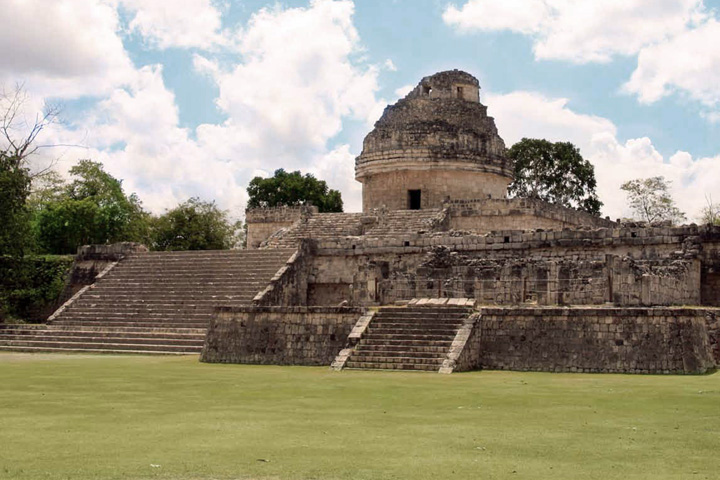
\includegraphics[width=\marginparwidth]{figures/caracol.jpg}
 % \label{fig:caracol}
%\end{marginfigure}





